\documentclass[11pt,a4paper]{article}

\usepackage[T1]{fontenc}
\usepackage[utf8]{inputenc}
\usepackage{libertinus}
\usepackage{microtype}
\usepackage[a4paper,top=28mm,bottom=30mm,left=31mm,right=31mm]{geometry}
\usepackage{mathtools,amssymb,amsthm,stmaryrd}
\usepackage{booktabs}
\usepackage{float}
\usepackage{enumitem}
\usepackage{array}
\usepackage{tabularx}
\usepackage{tikz}
\usetikzlibrary{arrows.meta,positioning,calc,fit}
\usepackage[hidelinks]{hyperref}
\usepackage{xcolor}
\usepackage{fancyhdr}
\usepackage{titlesec}

\definecolor{softgray}{gray}{0.45}
\definecolor{rulegray}{gray}{0.72}
\definecolor{boxgray}{gray}{0.96}

\hypersetup{
  pdftitle={Epistemic Dynamics under Inconsistency: Recovery, Active Experimentation, Model Criticism, and Rational Self-Trust in 4PEL},
  pdfauthor={Julian L. Voigt (cr4bbz)},
  pdfsubject={4PEL, epistemic dynamics, active sensing, model uncertainty, self-trust, model criticism, formal verification},
  pdfkeywords={4PEL, paraconsistent logic, epistemic dynamics, active sensing, Bayesian control, model uncertainty, model misspecification, rational self-trust, Lean 4}
}

\pagestyle{fancy}
\fancyhf{}
\fancyhead[L]{\small\textsc{Epistemic Dynamics under Inconsistency}}
\fancyhead[R]{\small\textsc{4PEL}}
\fancyfoot[C]{\small\thepage}
\renewcommand{\headrulewidth}{0.3pt}

\titleformat{\section}{\Large\bfseries}{\thesection}{0.75em}{}
\titleformat{\subsection}{\large\bfseries}{\thesubsection}{0.65em}{}
\titlespacing*{\section}{0pt}{2.4ex plus .6ex minus .2ex}{1.0ex}
\titlespacing*{\subsection}{0pt}{1.8ex plus .4ex minus .2ex}{.7ex}

\setlength{\parindent}{0pt}
\setlength{\parskip}{0.72em}
\setlist[itemize]{leftmargin=1.6em,itemsep=.25em,topsep=.4em}
\setlist[enumerate]{leftmargin=1.8em,itemsep=.3em,topsep=.4em}

\newtheorem{theorem}{Theorem}
\newtheorem{proposition}[theorem]{Proposition}
\newtheorem{corollary}[theorem]{Corollary}
\theoremstyle{definition}
\newtheorem{definition}[theorem]{Definition}
\newtheorem{remark}[theorem]{Remark}

\newcommand{\Recovery}{\mathsf{Rec}}
\newcommand{\NonRecovery}{\mathsf{NonRec}}
\newcommand{\ObsEq}{\mathrel{\sim_{\mathrm{obs}}}}
\newcommand{\Bel}{\mathsf{B}}
\newcommand{\Cond}[1]{\mathsf{C}_{#1}}
\newcommand{\PhiPot}{\Phi}
\newcommand{\rhoReg}{\rho}
\newcommand{\Gate}[1]{\textsc{Gate #1}}
\newcommand{\RobustRec}{\mathsf{RobustRec}}
\newcommand{\TruthAligned}{\mathsf{TruthAligned}}
\newcommand{\BeliefState}{\mathsf{Bel}}

\begin{document}

\begin{titlepage}
\thispagestyle{empty}
\vspace*{7mm}

{\fontsize{23}{27}\selectfont\bfseries Epistemic Dynamics under Inconsistency\par}
\vspace{3mm}
{\fontsize{15}{18}\selectfont Recovery, Active Experimentation, Model Criticism, and Rational Self-Trust in 4PEL\par}

\vspace{7mm}
{\large Julian L. Voigt \quad (cr4bbz)\par}
\vspace{2mm}
{\normalsize Research Paper v0.3.0 \quad 15 September 2026\par}

\vspace{7mm}
\hrule height 0.5pt
\vspace{5mm}

\begin{abstract}
This paper develops a formally verified account of epistemic dynamics under inconsistency within 4PEL, a four-valued epistemic framework combining paraconsistent semantic structure, probabilistic belief, modal evaluation, and explicit update dynamics. The original Recovery program is extended from passive revision to active epistemic agency and, finally, to model criticism directed at the agent's own information-generating machinery. The verified development now spans six connected layers. First, Recovery is path-dependent and can exhibit genuine hysteresis, while a state-sufficiency result shows that this path sensitivity need not require an additional history register. Second, information acquisition becomes a control problem: finite Bellman recursion, stochastic epistemic transition, value of information, regret, reward alignment, partial observation, Bayesian filtering, and noisy sensing are represented without identifying internal 4PEL probability with external transition or observation probability. Third, the agent chooses experiments rather than merely receiving signals. Structural observational aliases can survive arbitrarily many repetitions of an uninformative experiment, whereas an alternative diagnostic intervention breaks the alias; finite-horizon control then determines when to sense, when to stop, and when sensing cost crosses an exact phase boundary. Fourth, posterior evidence is bridged back into four-valued status. Contradiction can therefore become an explicit control state: a finite policy rationally pays to transform status $B$ into a determinate $T$ or $F$ outcome. Fifth, uncertainty is lifted from the world to the observation model itself. Bayesian model beliefs, calibration, robust maximin control, joint world--model posteriors, and a dual value-of-information problem allow one observation to update both first-order belief about the world and second-order trust in the sensor. In a concrete degraded-sensor witness, failed calibration changes the policy from a fragile action with objective value $1/10$ to a safe action with value $3/5$, eliminating regret from $1/2$ to $0$. Sixth, the framework crosses the closed-model boundary. A residual observation may be better explained by a model absent from the original class; sufficiently low predictive evidence triggers model doubt and an explicit action to expand the hypothesis space. Gates 101--104 then assign probability mass to an outside-class possibility, distinguish meta-level ignorance $N$ from contradiction $B$, represent world status and model status as independent four-valued axes, and define a finite self-trust controller that acts, calibrates, or expands its model class according to the meta-status of its own epistemic machinery. These results support a dynamic conception of rationality in which an agent can revise not only what it believes, but which experiment it performs, how much it trusts its evidence source, and whether its hypothesis class is adequate. All principal claims reported here are mechanized in Lean 4; claims of philosophical generality are kept separate from the verified finite witnesses.
\end{abstract}

\vspace{5mm}
\begin{center}
\footnotesize
\textbf{Status.} Independent research paper. The reported formal results are verified in Lean 4, but the paper has not undergone external peer review.\par
\vspace{2mm}
Formalization snapshot: \path{research/epistemic-self-trust-integration-gate104}, commit \path{2cf3c12db6aa222a92af2c512ae68aae3fb7a0df}.
\end{center}
\end{titlepage}

\pagenumbering{roman}
\begingroup
\small
\setlength{\parskip}{0pt}
\tableofcontents
\endgroup
\clearpage
\pagenumbering{arabic}

\section{Introduction}

Formal epistemology often begins with a state: a set of beliefs, a probability function, a Kripke model, or a theory closed under some consequence relation. The present project begins one step later. Its central question is not merely which epistemic states are acceptable, but which \emph{dynamics of change} make epistemic recovery possible when information is inconsistent, probabilistic, partially observed, and generated by mechanisms whose reliability is itself uncertain.

4PEL provides a useful environment for this question because contradiction is represented without immediate trivialization. An agent can occupy states in which positive and negative support coexist, while modal and probabilistic structure can still evolve. This separates phenomena that classical consistency-first accounts often place under one heading: being inconsistent now, being able to recover later, selecting which information to acquire, deciding whether to trust a sensor, and recognizing that the current model class may itself be inadequate.

The main claim of this paper is deliberately dynamic:

\begin{quote}
\textbf{Epistemic rationality can be studied as a property of learning, experimentation, calibration, and model-revision dynamics rather than solely as a property of instantaneous belief states.}
\end{quote}

The claim is not introduced as a philosophical stipulation. It is motivated by a sequence of machine-checked finite results. The development begins with Recovery variation, asymptotic stabilization, path dependence, and hysteresis. It isolates a confluent fragment of static evidence and a genuinely hysteretic regime generated by endogenous evidence. A state-sufficiency theorem then shows that history can matter through the current full model without requiring an additional history variable. Closed epistemic loops can return to the same Recovery status while leaving a nonzero full-model displacement, and oppositely composed anchored loops can fail to commute.

The second stage turns updates into actions. Once information acquisition is under agent control, \emph{being recovered} and \emph{learning well} come apart. A myopic Recovery reward can favor information avoidance, whereas a longer horizon can make temporary destabilization rational. Finite Bellman recursion, stochastic transition kernels, value of information, regret, and reward thresholds are then layered over the 4PEL dynamics. Partial observation adds a posterior over hidden epistemic states, and noisy observation makes Recovery a probabilistic signal rather than an oracle.

The third stage, new in v0.3.0, makes the experimental design itself endogenous. A controller may choose among observation channels with different likelihood profiles and costs. This exposes a fundamental distinction between \emph{more data} and \emph{more identifiability}: if two hidden states are observationally aliased under an experiment, arbitrarily many repetitions of that same experiment can leave the posterior split exactly unchanged. An alternative intervention can break the alias. The controller must therefore decide not only how long to observe, but \emph{what kind of observation to perform} and when additional information is no longer worth its cost.

The fourth and fifth stages turn this machinery reflexive. Posterior support is mapped back into the four values $T,F,B,N$, so contradiction and ignorance become control-relevant states rather than mere labels. Then uncertainty is lifted from the world to the observation model itself. An agent can be uncertain whether its sensor is reliable, update that uncertainty through calibration, and allow the resulting model posterior to change its next action. A joint posterior over world state and sensor model couples first-order and second-order uncertainty in one finite Bayesian state.

The final stage crosses the closed-model boundary. If every known model predicts an observation poorly, posterior reweighting within the known class may be the wrong operation. The formal development therefore introduces predictive surprise, model doubt, an explicit action to expand the hypothesis space, and finally an ``unknown'' probability mass. This yields a nested two-axis epistemic state
\[
  (\text{world status},\text{model status}) \in \{T,F,B,N\}^2,
\]
and a finite self-trust controller whose priority depends on the model-status coordinate. A trusted model licenses ordinary world-directed action; an ignorant model status triggers model expansion; contradictory or rejected model evidence triggers calibration.

Accordingly, the paper now studies a hierarchy of state descriptions:
\[
M_t
\quad\leadsto\quad
s_t
\quad\leadsto\quad
b_t
\quad\leadsto\quad
b_t^{\mathrm{world}\times\mathrm{model}}
\quad\leadsto\quad
(v^{\mathrm{world}}_t,v^{\mathrm{model}}_t).
\]
The first level carries 4PEL semantics, the second supports controlled hidden state, the third supports Bayesian control under partial observability, the fourth represents coupled uncertainty about world and sensor model, and the fifth compresses first- and second-order epistemic assessment into two four-valued coordinates. These levels are deliberately not identified with one another.

The principal contribution is therefore not a single universal optimality theorem. It is an executable and verified architecture that makes several boundaries explicit: Recovery versus truth, posterior uncertainty versus contradiction, repeated evidence versus identifiability, Bayesian optimism versus robust control, calibration versus world-directed sensing, and ordinary Bayesian updating versus structural model revision. The finite witnesses are strong enough to establish the possibility and internal consistency of these distinctions while leaving their generalization as an open mathematical program.

\section{Background and Scope}

\subsection{Four-valued epistemic states}

4PEL inherits the central insight of Belnap--Dunn four-valued semantics: positive and negative support need not be complements. A proposition may be supported positively, supported negatively, supported in both directions, or supported in neither direction. This supplies a paraconsistent semantic substrate in which inconsistency can be represented locally without validating arbitrary explosion \cite{belnap1977useful,dunn1976}.

The present paper does not reconstruct the complete 4PEL architecture. It uses only the following structural facts from the wider formalization:

\begin{itemize}
  \item formulas are evaluated in four-valued epistemic models;
  \item models contain probabilistic structure used to evaluate belief;
  \item evidence formulas can be used to Conditionalize the current model when admissibility conditions are satisfied;
  \item a compositional \emph{Recovery} predicate records when the relevant four-valued semantics supports a classical-like fragment for a target formula or modal expression.
\end{itemize}

Recovery is therefore a formal semantic property internal to the model. It must not be identified with correspondence truth. A recovered agent may still be factually wrong; conversely, a non-recovered state may encode genuine conflicting information about the world. The object studied here is the \emph{dynamics of Recovery}, not a general theory of truth.

\subsection{Updates and endogenous evidence}

Let $M$ be a current model and let $P$ be an admissible evidence formula. We write
\[
\Cond{P}(M)
\]
for the result of Conditionalization on the positive extension of $P$ in $M$.

A crucial distinction concerns how the relevant evidence event is obtained. For an atomic or otherwise belief-free formula, its extension is fixed by valuation and Boolean structure and is unaffected by a probability-only Conditionalization. By contrast, an evidence formula containing an epistemic belief operator can be \emph{endogenous}: its extension may depend on the probability distribution of the current model. Thus an earlier update can change what a later piece of syntactically identical evidence denotes.

This distinction separates the static and feedback regimes studied below.

\subsection{Formal method}

The results reported here were developed theorem-first in Lean 4. Countermodels and positive theorems are represented in the same environment. The formal workflow is deliberately adversarial: each proposed generalization is tested against explicit finite witnesses, and each philosophical interpretation is restricted to what the formal statement establishes.

The current snapshot is the 4PEL-Lean-Formalization repository at commit\
\begin{center}
\small\path{67f1187d4b64f77c43289999c4e22b004a3dafa3}
\end{center}
The principal Lean modules for this paper are listed in Appendix A; they include the path-dependence, hysteresis, semantic-feedback, confluence, state-sufficiency, and tail-attractor developments \cite{repo2026}.

\section{From Recovery to Path-Dependent Dynamics}

\subsection{Finite variation is not attraction}

The early Recovery-dynamics results introduce a natural-valued potential $\Phi(s)$ on epistemic states. Under a basic descent contract, a change in Boolean Recovery status must consume potential. The immediate consequence is a finite variation principle: Recovery cannot flip infinitely often along a valid trajectory whose relevant potential is finite.

This already separates two questions:
\[
\text{Does the phase eventually stop changing?}
\qquad\text{and}\qquad
\text{Which phase is eventually reached?}
\]
A finite flip budget answers only the first. A trajectory may stabilize permanently in Recovery or permanently in Non-Recovery.

This distinction is methodologically important. Convergence of an observable is not yet convergence to an epistemically privileged observable value.

\subsection{Path dependence from one recovered start}

\Gate{29} establishes a stronger result. There exists a single recovered 4PEL model with two admissible evidence futures whose asymptotic Recovery phases differ. In the concrete witness, learning one atomic proposition selects a fixed point that remains recovered; learning another selects a fixed point that remains non-recovered. Repeating the same admissible atomic evidence is idempotent after the first update.

\begin{proposition}[Path-dependent Recovery phase]
There is a recovered model $M_0$ and two admissible update schedules $\sigma_1,\sigma_2$ such that the corresponding trajectories begin at the same $M_0$, while one is eventually permanently recovered and the other eventually permanently non-recovered.
\end{proposition}

The proposition separates three notions:
\begin{enumerate}
  \item Recovery now;
  \item eventual Recovery along one admissible future;
  \item Recovery under all admissible futures.
\end{enumerate}
The first does not imply the third. Recovery is therefore not, by itself, a guarantee about the future selected by later evidence.

\subsection{Recovery as an epistemic attractor}

\Gate{32} asks what additional structure is sufficient to select Recovery as the eventual phase. The answer uses two local conditions on a descent system:

\begin{align*}
\text{Recovery absorption:}\quad
&\Recovery(s)\land s\to t \Longrightarrow \Recovery(t),\\[2mm]
\text{Non-Recovery consumption:}\quad
&\neg\Recovery(s)\land s\to t \Longrightarrow \Phi(t)<\Phi(s).
\end{align*}

\begin{theorem}[Finite Recovery attraction]
If Recovery is absorbing and every Non-Recovery transition strictly decreases a natural-valued potential, then every valid trajectory reaches permanent Recovery in at most $\Phi(s_0)$ steps:
\[
\exists N\leq \Phi(s_0)\;\forall n\geq N:\;\Recovery(s_n).
\]
\end{theorem}

The potential now has a stronger interpretation than a mere flip budget. Under the attractor contract it behaves as a distance-like resource: remaining outside Recovery costs finite epistemic capacity.

The theorem is conditional. Arbitrary 4PEL Conditionalization does not satisfy Recovery absorption, as the path-dependence witness itself demonstrates. The result instead identifies a structural contract under which Recovery becomes a quantitative attractor.

\section{Hysteresis from Endogenous Evidence}

\subsection{The Gate-33 witness}

Path dependence does not yet amount to hysteresis. A stronger question holds the evidence ingredients fixed and changes only their order. \Gate{33} supplies such a witness with the pair $\{e,\Bel p\}$.

Initially the positive extension of $\Bel p$ contains all three relevant worlds. After conditioning on $e$, the belief profile changes, and the positive extension of the \emph{same syntactic evidence formula} $\Bel p$ shrinks. Consequently,
\[
\Cond{e}(\Cond{\Bel p}(M_0))
\quad\text{and}\quad
\Cond{\Bel p}(\Cond{e}(M_0))
\]
have different Recovery outcomes.

\begin{proposition}[Endogenous-evidence hysteresis]
There is a model $M_0$ and two admissible evidence formulas $e$ and $\Bel p$ such that reversing their order changes the final Recovery judgment:
\[
\neg\Recovery(\Bel p;e)
\qquad\text{but}\qquad
\Recovery(e;\Bel p).
\]
\end{proposition}

The result must be interpreted carefully. It does \emph{not} show that two fixed extensional events fail to commute. Rather, the evidence language can inspect the evolving epistemic model, and the first update changes the event denoted by the second formula. The source of hysteresis is therefore semantic feedback.

\subsection{Regenerative Recovery budgets}

Hysteresis motivates a second relaxation. If epistemic updates can reveal or create new relevant structure, a fixed initial flip budget may be too restrictive. \Gate{34} introduces a regeneration term $\rho(s,t)$ and replaces pure descent with a balance law:
\[
 c(s,t)+\Phi(t)\leq \Phi(s)+\rho(s,t),
\]
where $c(s,t)$ is the unit cost of a Recovery-status change.

Along a finite path this telescopes to
\[
\#\text{Recovery changes}+\Phi_{\mathrm{final}}
\leq
\Phi_{0}+\sum \rho.
\]
Hence
\[
\boxed{
\#\text{Recovery changes}
\leq
\Phi_{0}+\text{total regeneration}.
}
\]

The zero-regeneration case recovers the earlier finite-descent theory. The conceptual shift is from a depleting counter to a balance sheet. A Recovery transition that could not be financed by the original potential may still occur if earlier updates regenerate resource.

Unbounded regeneration destroys the stabilization guarantee. This observation becomes decisive in the open problem of growing ontologies discussed in Section~\ref{sec:open}.

\section{The Confluence Boundary}

\subsection{Belief-free evidence is extension-stable}

\Gate{36} defines a recursively belief-free fragment of the evidence language. Conditionalization changes the probability measure but leaves the atomic valuation and accessibility structure fixed. Structural induction therefore yields exact evaluation stability for belief-free formulas. Their positive evidence extensions do not change under prior Conditionalization.

In schematic form,
\[
\mathsf{BeliefFree}(P)
\Longrightarrow
\llbracket P\rrbracket^+_{\Cond{Q}(M)}
=
\llbracket P\rrbracket^+_M.
\]

This gives a syntactically identifiable region in which the Gate-33 feedback mechanism cannot arise.

\subsection{Static schedule confluence}

\Gate{38} lifts this stability from single formulas to finite schedules. For arbitrary belief-free formulas $P$ and $Q$, under finite probability integrity and the required sequential admissibility conditions,
\[
\Cond{P}(\Cond{Q}(M))
\ObsEq
\Cond{Q}(\Cond{P}(M)),
\]
where $\ObsEq$ denotes modal observational equivalence.

Moreover, observational equivalence is preserved under a common admissible belief-free suffix. Thus an adjacent swap inside a finite static schedule preserves every modal value and every derived compositional Recovery judgment, provided both reordered executions remain admissible.

This yields a local generator for permutation confluence. It also reveals the beginnings of an update algebra: atomic repetition is idempotent, and belief-free updates commute observationally under the stated conditions.

\begin{figure}[ht]
\centering
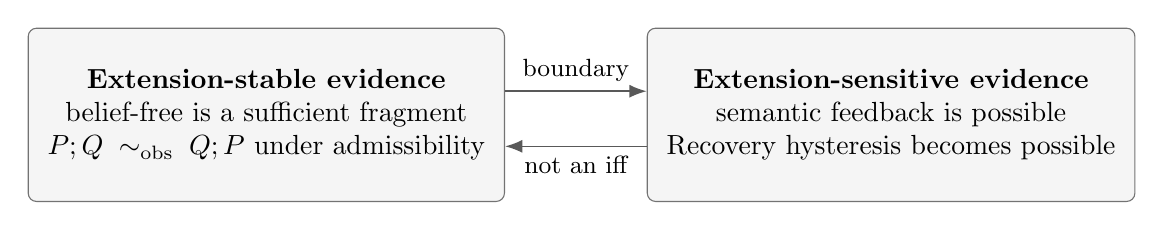
\begin{tikzpicture}[
  node distance=12mm,
  big/.style={draw=black!55, rounded corners=3pt, fill=boxgray, align=center, minimum width=58mm, minimum height=22mm, inner sep=7pt},
  arr/.style={-{Latex[length=2.2mm]}, semithick, draw=black!65}
]
\node[big] (static) {\textbf{Extension-stable evidence}\\belief-free is a sufficient fragment\\$P;Q\;\ObsEq\;Q;P$ under admissibility};
\node[big, right=18mm of static] (feedback) {\textbf{Extension-sensitive evidence}\\semantic feedback is possible\\Recovery hysteresis becomes possible};
\draw[arr] ($(static.east)+(0,3mm)$) -- node[above, font=\small]{boundary} ($(feedback.west)+(0,3mm)$);
\draw[arr] ($(feedback.west)+(0,-4mm)$) -- node[below, font=\small]{not an iff} ($(static.east)+(0,-4mm)$);
\end{tikzpicture}
\caption{The verified phase boundary. Belief-free syntax guarantees extension stability, but belief-containing syntax does not by itself imply sensitivity.}
\label{fig:boundary}
\end{figure}

\subsection{A semantic no-go theorem for hysteresis}

\Gate{40} removes the remaining syntactic ambiguity. Let $P$ and $Q$ be arbitrary evidence formulas, possibly containing belief operators. Suppose their positive extensions are mutually stable under the opposite update. Under probability integrity and mutual sequential admissibility, the two update orders are modally observationally equivalent and therefore Recovery-confluent.

\begin{theorem}[Strong hysteresis boundary]
If $P$ is extension-stable under the update by $Q$ and $Q$ is extension-stable under the update by $P$, then
\[
P;Q\ObsEq Q;P,
\]
and all current modal Recovery judgments agree at the two endpoints.
\end{theorem}

Taking the contrapositive yields the central diagnostic:
\[
\boxed{
\text{Recovery hysteresis}
\Longrightarrow
\text{semantic extension feedback in at least one direction}.
}
\]

Thus the presence of a belief operator is not the explanatory primitive. A belief-containing formula may remain extension-stable in a particular model. The verified necessary condition is semantic, not merely syntactic. Feedback is necessary for the formal two-update Recovery hysteresis result, but it is not sufficient by itself.

\section{History Sensitivity without a History Register}

Hysteresis naturally raises a memory question. If update order matters, must the formal state contain an explicit record of the past?

\Gate{39} answers negatively for Conditionalization. A finite schedule-run object allows arbitrary evidence formulas, including belief-dependent evidence. The next model is determined by the current full model, the next syntactic evidence formula, and an admissibility proof. Proof irrelevance prevents different admissibility witnesses from encoding hidden dynamics.

\begin{theorem}[Epistemic state sufficiency]
For arbitrary admissible Conditionalization schedules,
\[
\boxed{
\text{same current full model}
+
\text{same future evidence schedule}
\Longrightarrow
\text{same endpoint full model}.
}
\]
\end{theorem}

Two histories that merge at exactly the same current model therefore coalesce under every common admissible future schedule. Since endpoint model equality implies agreement on subsequent modal values and Recovery judgments, the full current model is a sufficient statistic for the represented update dynamics.

This reconciles path dependence with a Markov-style interpretation:
\[
\text{history}
\longrightarrow
\text{different present model}
\longrightarrow
\text{different future semantics}.
\]
No additional memory variable is required. The past matters precisely insofar as it has become present structure.

The qualification \emph{full model} is essential. Recovery status alone is too coarse. Two states can share the same current Boolean Recovery phase while encoding probability distributions or belief extensions that make their future behavior diverge.

\section{Control, Filtering, and Decision-Theoretic Epistemics}

This section collects the four previously separated developments on recovery loops, active control, decision theory, and the distinction between truth-directed internal belief and stochastic external dynamics. The subdivision is intentionally modular so that each formal layer remains auditable against its Lean source.

\section{Recovery after Semantic Turbulence}

The preceding results create an apparent tension. The framework admits path dependence, semantic feedback, hysteresis, and regeneration. Why should Recovery ever be permanent?

\Gate{41} resolves the tension by separating the past from the tail of a realized trajectory.

\subsection{A cutoff theorem}

Consider a regenerative Recovery system with status function, natural-valued potential $\Phi$, regeneration function $\rho$, and a realized infinite trajectory $s_0,s_1,\ldots$. Fix a cutoff time $K$. Assume only that the following three conditions hold from $K$ onward:

\begin{enumerate}
  \item \textbf{Regeneration ceases}: every realized tail transition has $\rho=0$.
  \item \textbf{Recovery is absorbing on the realized tail}: once Recovery is reached, the next realized state is also recovered.
  \item \textbf{Non-Recovery consumes potential}: each realized transition beginning in Non-Recovery strictly lowers $\Phi$.
\end{enumerate}

No corresponding restrictions are imposed on the prefix before $K$. It may contain Recovery loss, Recovery restoration, semantic feedback, and resource regeneration.

\begin{theorem}[Recovery after semantic feedback]
Under the three tail conditions above, there exists $N$ such that
\[
K\leq N\leq K+\Phi(s_K)
\]
and
\[
\forall n\geq N:\quad \Recovery(s_n).
\]
Equivalently,
\[
\boxed{
T_{\mathrm{permanent\ Recovery}}
\leq K+\Phi(s_K).
}
\]
\end{theorem}

The proof compiles the realized tail into a time-indexed ordinary descent system. Because tail regeneration is zero, the regenerative budget collapses to the earlier descent inequality. The two remaining assumptions become exactly the Recovery-attractor contract. The earlier attractor theorem can therefore be reused rather than reproved.

This proof architecture matters conceptually. The theorem is path-local: it does not require every transition admitted by the ambient update system to be attractive. Only the realized future after $K$ must enter the dissipative regime.

\subsection{Sharpness}

The formalization contains a four-state witness:
\[
\begin{aligned}
\textsf{start}(\Recovery,\Phi=1)
&\to \textsf{fractured}(\NonRecovery,\Phi=1)\\
&\to \textsf{cutoff}(\NonRecovery,\Phi=1)\\
&\to \textsf{recovered}(\Recovery,\Phi=0).
\end{aligned}
\]
The first transition regenerates one resource unit and finances an early loss of Recovery. The cutoff is $K=2$. Permanent Recovery begins at time $3$, exactly saturating the bound:
\[
3=2+1=K+\Phi(s_K).
\]
The numerical bound is therefore sharp for the verified witness.

\begin{figure}[ht]
\centering
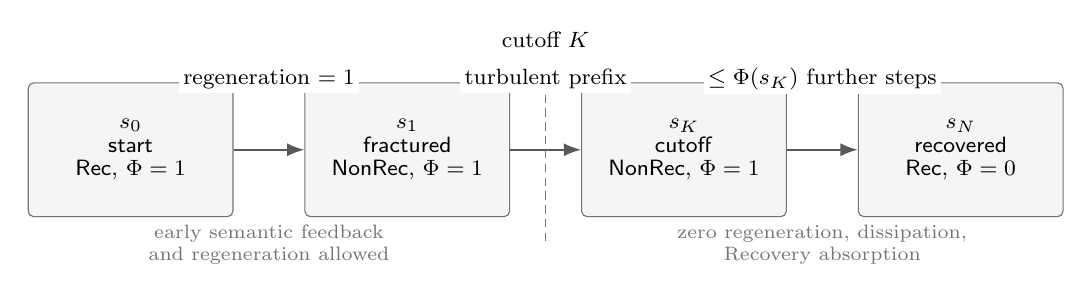
\begin{tikzpicture}[
  state/.style={draw=black!55, rounded corners=2pt, fill=boxgray, align=center,
    inner xsep=4pt, inner ysep=4.5pt, minimum width=26mm, minimum height=17mm,
    font=\footnotesize},
  arr/.style={-{Latex[length=2.2mm]}, semithick, draw=black!65},
  note/.style={font=\footnotesize, align=center, fill=white, inner sep=1.5pt},
  node distance=9mm
]
\node[state] (s0) {$s_0$\\[-1pt]\textsf{start}\\[-1pt]$\Recovery$, $\Phi=1$};
\node[state, right=of s0] (s1) {$s_1$\\[-1pt]\textsf{fractured}\\[-1pt]$\NonRecovery$, $\Phi=1$};
\node[state, right=of s1] (sk) {$s_K$\\[-1pt]\textsf{cutoff}\\[-1pt]$\NonRecovery$, $\Phi=1$};
\node[state, right=of sk] (sn) {$s_N$\\[-1pt]\textsf{recovered}\\[-1pt]$\Recovery$, $\Phi=0$};

\draw[arr] (s0) -- (s1);
\draw[arr] (s1) -- (sk);
\draw[arr] (sk) -- (sn);

\node[note] at ($(s0)!0.5!(s1)+(0,9mm)$) {regeneration $=1$};
\node[note] at ($(s1)!0.5!(sk)+(0,9mm)$) {turbulent prefix};
\node[note] at ($(sk)!0.5!(sn)+(0,9mm)$) {$\leq \Phi(s_K)$ further steps};

\coordinate (cut) at ($(s1)!0.5!(sk)$);
\draw[densely dashed, black!55] ($(cut)+(0,7mm)$) -- ($(cut)+(0,-12mm)$);
\node[note] at ($(cut)+(0,14mm)$) {cutoff $K$};

\node[font=\scriptsize, text=softgray, align=center] at ($(s0)!0.5!(s1)+(0,-12mm)$)
  {early semantic feedback\\and regeneration allowed};
\node[font=\scriptsize, text=softgray, align=center] at ($(sk)!0.5!(sn)+(0,-12mm)$)
  {zero regeneration, dissipation,\\Recovery absorption};
\end{tikzpicture}
\caption{Gate 41 restarts the epistemic accounting clock at the cutoff. The prefix may be hysteretic and regenerative; the tail must be dissipative. In the sharp witness, $K=2$ and permanent Recovery occurs at $N=3=K+\Phi(s_K)$.}
\label{fig:cutoff}
\end{figure}


\section{Closed Epistemic Loops and Discrete Curvature}

The Gate-41 cutoff result establishes that a turbulent past can be followed by a dissipative Recovery tail. Gates 42 and 43 ask a different question: what can remain when a control sequence returns syntactically to where it started?

\subsection{Recovery closure without full-state closure}

An \emph{evidence-control loop} first enters an anchor formula $P$, performs an excursion through $Q$, and returns to the same syntactic anchor $P$. In the verified witness,
\[
P=\Bel p,
\qquad
Q=e.
\]
The observable Recovery trajectory is
\[
\Recovery\;\longrightarrow\;\NonRecovery\;\longrightarrow\;\Recovery.
\]
Thus Recovery closes. The full epistemic model does not. A fixed atomic evidence probe $E=\{a,b\}$ has mass
\[
\mu_{\mathrm{anchor}}(E)=\frac45,
\qquad
\mu_{\mathrm{return}}(E)=1,
\]
so the two anchor models are unequal.

\begin{theorem}[Control-loop displacement, Gate 42]
There exists a finite 4PEL evidence-control loop that returns to the same syntactic control anchor and the same Recovery status while failing to return to the same full epistemic model.
\end{theorem}

The result is a stronger form of hysteresis than a single order-sensitive pair. The memory of the loop is stored in the displaced present model, not in an additional history register. This boundary is exact: if the loop returns to the identical full model, Gate 39 implies that every common admissible future schedule subsequently coalesces.

\subsection{Noncommuting loop composition}

Gate 43 composes two anchored excursions in opposite orders. Let $A$ be a neutral anchor in the concrete witness, with excursions $P=\Bel p$ and $Q=e$. The two schedules are schematically
\[
A\to P\to A\to Q\to A
\qquad\text{and}\qquad
A\to Q\to A\to P\to A.
\]
Their endpoints differ. Formally this yields a nonzero loop commutator,
\[
L_P\circ L_Q \neq L_Q\circ L_P,
\]
in the sense of unequal full epistemic endpoints.

\begin{theorem}[Discrete epistemic curvature witness, Gate 43]
There exists a finite anchored 4PEL loop pair whose opposite compositions are individually deterministic but terminate in different full epistemic models.
\end{theorem}

The geometric terminology is intentionally limited. This is a discrete noncommuting loop witness. No differentiable manifold, connection, curvature tensor, or holonomy group is claimed. Its significance is algebraic: semantic feedback can make the order of closed control excursions observable in the final epistemic state.

\section{From State Sufficiency to Active Epistemic Control}

\subsection{A Markov bridge on full models}

Gate 39 already states that the current full model is sufficient for fixed future schedules. Gate 44 packages the same idea as a controlled transition system. A state is a full 4PEL model $M$, an action is a syntactic evidence formula $a$, and an enabled one-step transition is a valid Conditionalization:
\[
M\xrightarrow{a}M'.
\]
The relation is deterministic whenever the action is admissible:
\[
M_1=M_2\ \land\ a_1=a_2
\quad\Longrightarrow\quad
M_1'=M_2'.
\]
Two different histories may therefore be compressed once they merge. The concrete witness compares $[p]$ with $[p,p]$: atomic idempotence makes the present models equal, and every common future action then has the same successor.

This is a \emph{Markov-like deterministic partial control system}, not yet an MDP. In particular, not every syntactic action is enabled in every state, and no reward or stochastic transition kernel is required at this stage.

\subsection{Choosing questions without choosing answers}

Gate 45 distinguishes an information-acquisition plan from its realized evidence. Plans include schematic actions such as observing $\varphi$, querying a source about $\varphi$, testing $\varphi$, or running an experiment. The agent can choose the plan, but need not control which evidential result it produces. In a polar acquisition semantics the same plan may realize either $\varphi$ or $\neg\varphi$.

This distinction blocks a common conflation in active epistemology: choosing to investigate is not choosing what the investigation will show. It also creates genuine control. From the same initial model, one admissible observation can preserve Recovery while another admissible probe destroys it. Thus an agent's evidence-selection policy can alter its Recovery trajectory.

\subsection{Reward misspecification and rational destabilization}

Gate 46 assigns a deliberately myopic reward to two available information choices:
\[
R_{\mathrm{now}}(a_{\mathrm{preserve}})=1,
\qquad
R_{\mathrm{now}}(a_{\mathrm{probe}})=0.
\]
Because the first choice preserves immediate Recovery and the second does not, the preserving action is uniquely myopically optimal. The formal point is not that the agent is irrational. The optimizer is correct relative to a poor proxy.

Gate 47 then separates ordinary Recovery from \emph{robust Recovery}. A fragile state can satisfy Recovery while failing an admissible stress test; a robust state satisfies Recovery and preserves it across the designated stress relation. The verified paths have the schematic form
\[
\begin{array}{rcl}
\text{preserve:}& \Recovery&\to\Recovery\to\Recovery\to\cdots\quad\text{but fragile},\\[1mm]
\text{probe:}& \Recovery&\to\NonRecovery\to\NonRecovery\to\Recovery\quad\text{and robust}.
\end{array}
\]
Consequently,
\[
a_{\mathrm{preserve}}\succ_1 a_{\mathrm{probe}},
\qquad
 a_{\mathrm{probe}}\succ^{\mathrm{robust}}_3 a_{\mathrm{preserve}}.
\]
The preference reversal verifies a minimal form of \emph{rational destabilization}: temporary loss of a coarse epistemic status can be required by a longer-horizon robustness objective.

\subsection{Exploration has a deadline}

Gate 48 repeats the choice through an \textsf{exploit}/\textsf{explore} controller. Exploitation remains in the fragile Recovery basin. Exploration enters the destabilized path and requires time to integrate. In the three-step witness,
\[
[\textsf{explore},\textsf{exploit},\textsf{exploit}]
\longrightarrow \textsf{robust},
\]
whereas
\[
[\textsf{exploit},\textsf{explore},\textsf{exploit}]
\longrightarrow \textsf{integrating}.
\]
More strongly, any three-action run that reaches the robust state must choose \textsf{explore} first. Information acquisition therefore has not only value but \emph{lead time}: delaying a good experiment can make a robustness deadline unreachable.

\begin{figure}[ht]
\centering
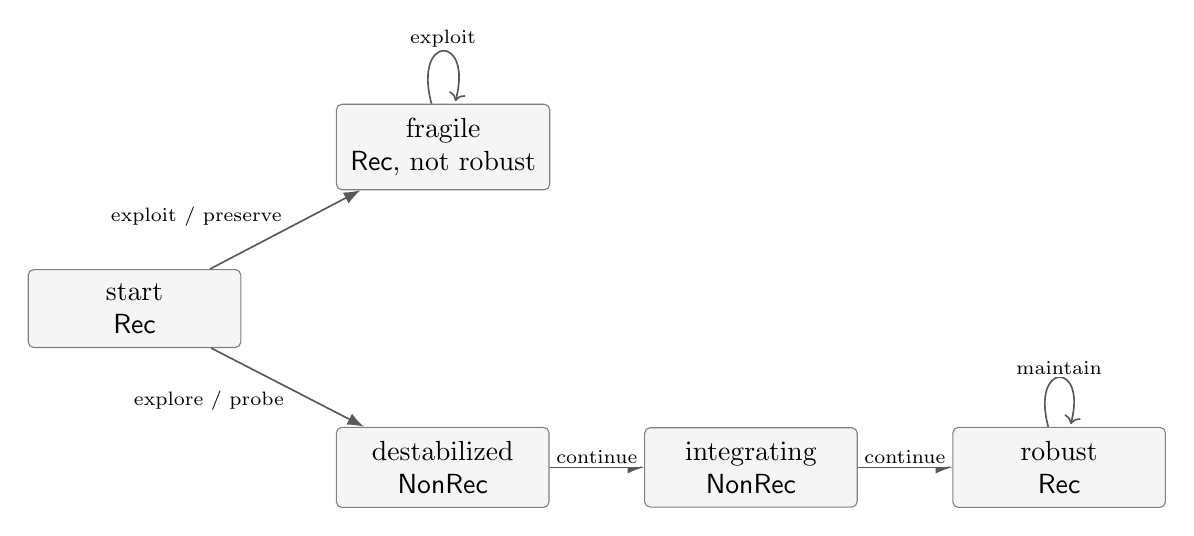
\begin{tikzpicture}[
  st/.style={draw=black!50, rounded corners=2pt, fill=boxgray, align=center, inner sep=5pt, minimum width=27mm},
  arr/.style={-{Latex[length=2.1mm]}, semithick, draw=black!65},
  lab/.style={font=\scriptsize, fill=white, inner sep=1pt},
  node distance=10mm and 12mm
]
\node[st] (start) {start\\$\Recovery$};
\node[st, above right=of start] (frag) {fragile\\$\Recovery$, not robust};
\node[st, below right=of start] (dest) {destabilized\\$\NonRecovery$};
\node[st, right=of dest] (integ) {integrating\\$\NonRecovery$};
\node[st, right=of integ] (rob) {robust\\$\Recovery$};
\draw[arr] (start) -- node[lab, above left] {exploit / preserve} (frag);
\draw[arr] (frag) edge[loop above] node[lab] {exploit} (frag);
\draw[arr] (start) -- node[lab, below left] {explore / probe} (dest);
\draw[arr] (dest) -- node[lab, above] {continue} (integ);
\draw[arr] (integ) -- node[lab, above] {continue} (rob);
\draw[arr] (rob) edge[loop above] node[lab] {maintain} (rob);
\end{tikzpicture}
\caption{The finite control witness underlying Gates 46--48. Immediate Recovery favors the upper path; robust Recovery under a deadline favors immediate exploration along the lower path.}
\label{fig:control-witness}
\end{figure}

\section{Finite Epistemic Decision Theory}

Gates 49--53 convert the preceding witness into explicit finite decision-theoretic objects. The purpose is not to claim that 4PEL is intrinsically an MDP. Rather, it is to show that its verified epistemic dynamics can support controlled optimization once actions, transition uncertainty, and objectives are added explicitly.

\subsection{Bellman recursion and stochastic transition}

Gate 49 defines a finite epistemic decision process and a finite-horizon Bellman recursion. In the concrete witness, horizon one favors exploitation, while horizon three favors exploration. The latter is no longer stipulated as the preferred policy: it attains the computed Bellman optimum, with
\[
V_3(\textsf{start})=4.
\]
Thus the earlier preference reversal emerges from dynamic programming rather than from a hand-selected trajectory.

Gate 50 introduces an external stochastic transition kernel over epistemic states. The distinction from the internal 4PEL probability is essential:
\[
\underbrace{P(w\mid M)}_{\text{uncertainty represented inside a 4PEL model}}
\qquad\neq\qquad
\underbrace{P(M'\mid M,a)}_{\text{uncertainty about the next epistemic state}}.
\]
In the finite stochastic witness, exploration branches with equal transition weight between a robust and a broken outcome, yet its expected continuation value still exceeds the safe alternative.

\subsection{Value of information and regret}

Gate 51 isolates the value of observing which branch occurred. Without the observation, the agent must choose one fixed response for both possible outcomes and can achieve value $5$. With the observation, it can condition its response on the realized state and achieve value $8$:
\[
\operatorname{VoI}=8-5=3>0.
\]
The information is valuable because it enables contingent action, not because information is postulated to possess an intrinsic positive reward.

Gate 52 measures epistemic regret against the Bellman optimum. Immediate exploration has regret $0$, delayed exploration has regret $3$, and persistent exploitation has regret $1$ in the verified witness. Timing is therefore part of epistemic performance: the same exploratory action can be optimal now and suboptimal one step later because integration consumes the remaining horizon.

\subsection{A reward-alignment threshold}

Gate 53 separates the reward for ordinary Recovery, $r$, from an additional robust-Recovery bonus, $b$. In the three-step witness, immediate exploration receives $r+b$, while persistent exploitation receives $3r$. Lean verifies the sufficient threshold
\[
\boxed{b>2r\quad\Longrightarrow\quad \textsf{explore}\succ\textsf{exploit}.}
\]
At or below the threshold exploitation is not worse in this witness. This is a finite reward-design result, not a universal theorem that one scalar reward captures epistemic rationality. It nevertheless formalizes a central warning: changing only the optimizer is unnecessary when the failure is caused by the objective it optimizes.

\section{Truth Calibration and Partial Observation}

The decision-theoretic extension makes an older boundary unavoidable. If Recovery is used as a reward, what relation does Recovery bear to truth? Gates 54--57 address this question without identifying the two notions.

\subsection{A conditional bridge from robust Recovery to truth alignment}

Gate 54 introduces an external calibration error together with a diagnostic-completeness condition. Every remaining positive calibration error must be exposable by at least one admissible stress test, and zero calibration error must imply an externally supplied predicate $\TruthAligned$. Under these assumptions,
\[
\RobustRec(s)
\quad\Longrightarrow\quad
\operatorname{calibrationError}(s)=0
\quad\Longrightarrow\quad
\TruthAligned(s).
\]
The assumptions do real work. Ordinary Recovery alone does not imply truth alignment: the formal \textsf{fragile} state is a counterexample. The theorem is therefore a bridge under explicit diagnostic conditions, not a redefinition of Recovery as truth.

\subsection{Why the visible Recovery bit is not a sufficient state}

Gate 55 makes the hidden-state problem explicit. The states \textsf{fragile} and \textsf{robust} can generate the same visible observation, \textsf{recovery}, while differing in calibration error, truth alignment, and stress robustness. Worse, the same visible observation followed by the same action can produce different next observations:
\[
\textsf{fragile}\xrightarrow{\textsf{explore}}\textsf{destabilized}\mapsto\textsf{nonRecovery},
\]
while
\[
\textsf{robust}\xrightarrow{\textsf{explore}}\textsf{robust}\mapsto\textsf{recovery}.
\]
Thus the Recovery observation is not Markov-sufficient for control. Partial observability is not merely imported by analogy; it is forced by a verified aliasing witness.

\subsection{A finite epistemic POMDP and normalized belief states}

Gate 56 packages hidden epistemic states, actions, stochastic transitions, and observations into a finite epistemic POMDP kernel. Its initial belief after observing only Recovery can leave both \textsf{fragile} and \textsf{robust} possible. An active probe changes the hidden-state distribution, after which the next observation filters the possible states.

Gate 57 normalizes these weights into rational Bayesian beliefs. Starting from
\[
b_0=\frac12\delta_{\textsf{fragile}}+\frac12\delta_{\textsf{robust}},
\]
exploration predicts
\[
\widehat b=\frac12\delta_{\textsf{destabilized}}+\frac12\delta_{\textsf{robust}}.
\]
Under the deterministic observation channel used at this stage,
\[
P(\textsf{recovery}\mid\textsf{explore})=\frac12,
\qquad
P(\textsf{nonRecovery}\mid\textsf{explore})=\frac12,
\]
and the corresponding posteriors collapse to the point masses $\delta_{\textsf{robust}}$ and $\delta_{\textsf{destabilized}}$. The hidden POMDP can therefore be read as a fully observed controlled process over belief states.

\section{Bayesian Filtering with Noisy Epistemic Sensors}

Gates 58--61 replace witness-specific belief manipulation with a more general finite filtering foundation.

\subsection{Generic normalization and canonical belief identity}

Gate 58 proves generic rational normalization for finite beliefs of nonzero total mass:
\[
\operatorname{Mass}(b)\neq0
\quad\Longrightarrow\quad
\operatorname{Mass}(\operatorname{Normalize}(b))=1.
\]
Zero mass is preserved as the representation of an impossible observation rather than being assigned an arbitrary posterior.

Gate 59 then separates storage syntax from epistemic identity. For example,
\[
[(1/2,s),(1/2,s)]
\qquad\text{and}\qquad
[(1,s)]
\]
are different lists but represent the same distribution. Belief equivalence is defined extensionally by aggregate weight at every hidden state:
\[
b_1\equiv b_2
\quad\Longleftrightarrow\quad
\forall s\; W_{b_1}(s)=W_{b_2}(s).
\]
A canonical profile removes duplicate-list artifacts from the controller state.

\subsection{Noisy Recovery signals}

Gate 60 replaces the deterministic observation map by a stochastic observation kernel $P(o\mid s)$. The model now contains three probabilistic levels that must remain distinct:
\[
P(w\mid M),
\qquad
P(s'\mid s,a),
\qquad
P(o\mid s').
\]
The first is internal 4PEL uncertainty over worlds, the second is transition uncertainty over hidden epistemic states, and the third is sensor uncertainty.

In the finite noisy witness, a Recovery signal is correct with likelihood $9/10$ for the robust branch and misleading with likelihood $1/10$ for the destabilized branch. From an equal predicted prior, observing Recovery yields
\[
P(\textsf{robust}\mid\textsf{recovery})=\frac9{10},
\qquad
P(\textsf{destabilized}\mid\textsf{recovery})=\frac1{10}.
\]
Hence
\[
\boxed{\text{Recovery is evidence for robustness, not an oracle for robustness.}}
\]

\subsection{Posterior sufficiency}

Gate 61 is the partially observable analogue of Gate 39. Under a fixed transition and observation model, if two histories produce the same current posterior and are followed by the same future action--observation sequence, their future posteriors coincide:
\[
\boxed{
 b_t^{(1)}=b_t^{(2)}
 +\text{ same future action--observation sequence}
 \Longrightarrow
 b_{t+n}^{(1)}=b_{t+n}^{(2)}.
}
\]
The result also respects Gate-59 equivalence: syntactically different belief lists that assign the same aggregate mass to every hidden state map to the same canonical controller state. The posterior is therefore a compressed epistemic memory for the encoded filter model.

This sufficiency claim is model-relative. If the transition kernel, observation kernel, or hidden-state ontology is misspecified, the theorem still describes the encoded filter but does not guarantee empirical adequacy.

\begin{figure}[ht]
\centering
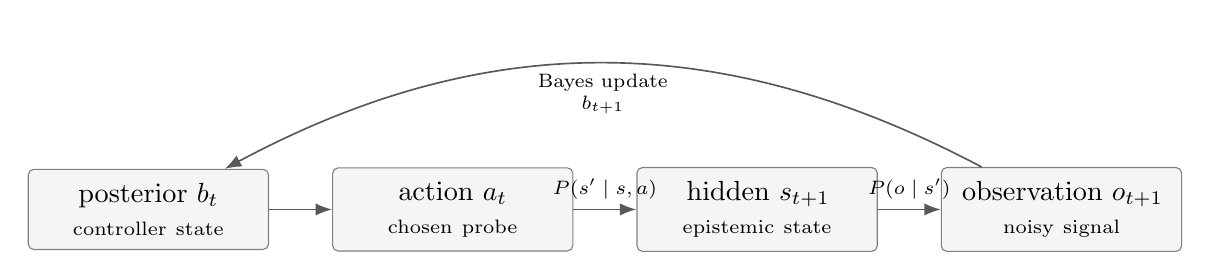
\begin{tikzpicture}[
  box/.style={draw=black!50, rounded corners=2pt, fill=boxgray, align=center, inner sep=5pt, text width=27mm},
  arr/.style={-{Latex[length=2.1mm]}, semithick, draw=black!65},
  node distance=8mm and 8mm
]
\node[box] (belief) {posterior $b_t$\\\scriptsize controller state};
\node[box, right=of belief] (act) {action $a_t$\\\scriptsize chosen probe};
\node[box, right=of act] (hidden) {hidden $s_{t+1}$\\\scriptsize epistemic state};
\node[box, right=of hidden] (obs) {observation $o_{t+1}$\\\scriptsize noisy signal};
\draw[arr] (belief) -- (act);
\draw[arr] (act) -- node[above, font=\scriptsize] {$P(s'\mid s,a)$} (hidden);
\draw[arr] (hidden) -- node[above, font=\scriptsize] {$P(o\mid s')$} (obs);
\draw[arr] (obs) to[bend right=28] node[below, font=\scriptsize, align=center] {Bayes update\\$b_{t+1}$} (belief);
\end{tikzpicture}
\caption{The verified epistemic-control architecture through Gate 61. The controller acts on a posterior over hidden epistemic states. Transition uncertainty and observation noise are distinct from the probability represented internally by each 4PEL model.}
\label{fig:pomdp-loop}
\end{figure}


\section{Belief-State Control and Active Experiment Design}

Gates 62--69 continue the partial-observation program by moving Bellman control directly onto posterior states and then making the observation channel itself an object of choice. The shift is small syntactically but conceptually decisive: an epistemic controller is no longer restricted to choosing an external action after receiving evidence. It can choose \emph{which evidence-generating intervention to perform}.

\subsection{Bellman control on posterior states}

\paragraph{Lean-verified finite witness.}
Gate 62 defines a two-state belief controller over hidden \texttt{rest} and \texttt{stress} conditions. From the symmetric prior $(1/2,1/2)$, the immediate expected value of the recovery action is $2/5$, while the robust action has immediate value $7/10$. The encoded observation is informative: a positive signal yields posterior $(1/5,4/5)$ and a negative signal yields $(4/5,1/5)$. At horizon one the verified values are
\[
V_1(\mathsf{recovery})=\frac{21}{25},
\qquad
V_1(\mathsf{robust})=\frac{21}{20},
\]
so the Bellman controller selects the robust action.

\paragraph{Interpretation.}
The result closes the gap left at Gate 61. Posterior sufficiency is not merely a filtering theorem; the posterior can serve directly as the state of a decision process. The controller can therefore be memoryless with respect to raw observation history while still acting on everything in that history that is decision-relevant under the encoded model.

\subsection{Information can be informative and still not be worth buying}

\paragraph{Lean-verified finite witness.}
Gate 63 adds a meta-action between \texttt{sense} and \texttt{commit}. Immediate commitment has value $7/10$. Sensing costs $1/5$; after accounting for the downstream contingent response, its net value at the prior is $17/25$, strictly below $7/10$. The controller therefore commits rather than senses in the witness. The same dominance persists at the stressed posterior.

\paragraph{Interpretation.}
The theorem separates three claims that are easily conflated: a signal can be statistically informative, it can change the posterior, and yet it can have non-positive net decision value once cost is included. ``More information'' is not itself the objective of the control problem.

\subsection{Identifiability is structural, not a synonym for sample size}

Gate 64 defines observational equivalence through equality of likelihood profiles. In the verified three-state witness, \texttt{stressA} and \texttt{stressB} are aliases: starting from a $(1/2,1/2)$ posterior over the pair, either positive or negative observation leaves the posterior split unchanged. Gate 65 then introduces two experiments. A coarse experiment assigns likelihood $1/2$ in either hidden state and therefore preserves the alias, while a diagnostic experiment uses likelihoods $9/10$ and $1/10$. A positive diagnostic signal yields posterior $9/10$ on the first state, while a negative signal yields $1/10$.

Gate 66 sharpens the point by repetition. For every encoded repetition count, repeated positive evidence from the coarse experiment leaves the posterior at $1/2$. Repeating the diagnostic evidence instead produces
\[
\frac12,
\quad \frac9{10},
\quad \frac{81}{82},
\quad \frac{729}{730}
\]
after zero, one, two, and three positive observations. Gate 67 turns this contrast into an experiment-design result: structural aliasing cannot be repaired by taking more samples from an experiment that assigns equal likelihoods to the aliased states, but an intervention with unequal likelihoods can break it.

\begin{quote}
\textbf{Verified lesson: more data does not imply more identifiability. Sometimes the missing resource is not sample size but a different experiment.}
\end{quote}

\subsection{Adaptive experiments and an explicit stopping decision}

Gate 68 makes experiment selection belief-dependent: the informative probe is selected near the aliased posterior, while a cheaper action can be preferred once the state has been sufficiently resolved. Gate 69 adds a finite-horizon Bellman controller with an explicit \texttt{stop} action. At the alias, stopping has value $1/2$. The stress-oriented experiment has gross value $9/10$, cost $1/5$, and net value $7/10$. Horizon zero therefore stops, while horizons one and two select the experiment at the alias; after the informative result has moved the posterior into a resolved region, the verified controller stops.

\paragraph{Interpretation.}
This is the first point in the chain at which inquiry itself has an endogenous boundary. The agent chooses what to test, but also when the expected improvement no longer justifies another test. Epistemic agency is therefore not maximal curiosity. It is controlled allocation of information-gathering actions.


\section{Epistemic Agency and Four-Valued Contradiction Resolution}

Gates 70--77 analyze the geometry and economics of the active-sensing controller and then reconnect posterior control to the four-valued semantic layer.

\subsection{Cost phases, stopping regions, and dominance}

Gate 70 parameterizes sensing cost in hundredths. With gross experiment value $9/10$ and stopping value $1/2$, the exact critical cost is $40$ hundredths. The controller samples iff the cost is strictly below $40$; at exactly $40$ it stops. Thus the Gate-69 cost of $20$ lies inside the sampling region. Gate 71 packages this behavior as a stopping-region geometry: the aliased belief lies in the sampling region at the checked horizons, whereas the post-experiment resolved beliefs lie in the stopping region.

Gate 72 introduces experiment dominance. At the alias, the stress experiment $Q$-dominates the encoded cheaper and more precise alternatives for the checked horizons, and pruning the dominated actions preserves the Bellman value $7/10$. This is a finite computational witness that action-set simplification can preserve optimal value when dominance has been proved rather than assumed.

\subsection{Sequential identifiability and sample complexity}

Gate 73 uses four hidden states whose first and second bits are observed by separate diagnostics. Each diagnostic alone is non-identifying, but the pair is jointly identifying. Gate 74 quantifies the earlier diagnostic learning path. The posterior sequence
\[
\frac12,\frac9{10},\frac{81}{82},\frac{729}{730}
\]
crosses the encoded $90\%$ threshold after one positive observation, $98\%$ after two, and $99\%$ after three, while the $99.9\%$ target is not reached within the first three observations. The result is a concrete sample-complexity witness rather than an asymptotic rate theorem.

Gate 75 isolates a discounted Bellman fixed-point calculation. For
\[
T(v)=1+\frac12 v,
\]
the verified fixed point is $v=2$, and the residual of the finite iterates halves at each step. This provides a small exact bridge from finite-horizon calculations to fixed-point reasoning without claiming a general contraction theorem for all 4PEL controllers.

\subsection{From posterior support back to four values}

Gate 76 maps posterior support proposition-by-proposition into FDE status using the threshold $3/4$. The symmetric alias is classified as $N$, while the stress experiment drives the relevant posterior into determinate $T$ or $F$ outcomes. The posterior controller can therefore feed a four-valued semantic status rather than merely a scalar probability.

Gate 77 then begins from explicit contradiction: positive and negative support are both $4/5$, giving status $B$. Two possible resolution outcomes produce $T$ and $F$. Resolution utility is $1$ for determinate $T/F$ and $0$ for $B/N$; with cost $1/5$, the net value of resolving is $4/5$. The verified policy therefore chooses resolution, and every encoded resolution outcome exits $B$ into $T$ or $F$.

\paragraph{Interpretation.}
Paraconsistency prevents contradiction from exploding the theory, but Gate 77 adds a distinct claim: contradiction need not be inert. Once $B$ is part of a control state, an agent may rationally spend resources to transform contradictory evidence into a determinate outcome. Non-explosion and active contradiction management are compatible but conceptually different virtues.

\section{Model Uncertainty, Calibration, and Dual Epistemic Value}

The active-experimentation results still assume that the agent can treat its observation mechanism as known. Gates 78--94 relax that assumption. The resulting control problem has two coupled hidden objects: the state of the world and the quality of the model or sensor through which the world is observed. The formal development therefore separates first-order evidence from second-order trust rather than folding both into one scalar confidence value.

\subsection{From world uncertainty to model uncertainty}

The first move is to distinguish a probe's value under different sensor regimes. A robust action may remain useful across regimes while a fragile action can be excellent under a reliable sensor and poor under a degraded one. Model uncertainty therefore becomes decision relevant even when the first-order world question is unchanged.

Gates 80--85 connect this distinction back to four-valued evidence. In particular, a calibration problem can be represented as an epistemic gap rather than as an ordinary first-order falsehood, and a successful calibration can resolve the same initial state in different directions depending on the actual observation regime. These are finite witnesses rather than a general learning theory, but they establish the architectural point needed below: evidence about the world and evidence about the mechanism that generates world evidence need not be the same object.

\subsection{Bayesian model belief and calibration}

Gates 86--88 introduce explicit Bayesian belief over sensor models and an observation-driven posterior. This makes calibration an information-producing action rather than a purely logical rewrite. The action selected for the world can change because an observation changes belief about the model, even if the underlying world utility function itself is unchanged.

The relevant separation is
\[
\text{world-directed value}
\qquad\neq\qquad
\text{model-directed information value}.
\]
The posterior over the observation model is quantitative. Later four-valued meta-statuses therefore should not be read as replacements for the posterior; they are qualitative control summaries of a richer belief state.

\subsection{Joint world--model belief}

Gate 89 represents a joint distribution over world and model states rather than maintaining two unrelated marginals. Gate 90 then shows that two agents can have the same marginal belief about the world while selecting different actions because their model-trust marginals differ. This already anticipates the insufficiency result of Gate 107: a compressed epistemic label need not retain every distinction relevant to utility-optimal control.

Gate 91 gives world information and model information separate value terms. Gate 92 makes active calibration a competing action alongside acting immediately and sensing the world. In the encoded finite witness, calibration can have the highest net value because the same observation improves both model trust and downstream world control.

\subsection{Cost phase boundary and robust control}

Gate 93 varies calibration cost and produces an exact switching boundary between calibration and world sensing. The important result is structural rather than numerical: epistemic maintenance is an ordinary control action whose rationality depends on its expected value and cost.

Gate 94 adds a robustness comparison. A Bayesian policy can exploit a favorable model posterior, while a maximin policy may prefer a safe action under the same uncertainty. The formalization therefore keeps apart at least three questions:

\begin{enumerate}
  \item what the agent believes about the world;
  \item what the agent believes about the reliability of its own model;
  \item which decision criterion converts those beliefs into action.
\end{enumerate}

This distinction becomes essential in Gate 95. There the agent begins with an overconfident model belief, chooses the wrong action under the actual degraded sensor, receives corrective calibration evidence, and changes policy. The next section follows that self-correction beyond ordinary reweighting and into explicit criticism of the hypothesis class itself.

\paragraph{Boundary.}
The results summarized here are finite formal witnesses. They establish representational and control possibilities inside the encoded models; they do not by themselves prove generic Bayesian consistency, universal calibration optimality, or a privileged normative relationship between Bayesian and robust decision rules.

\section{Model Criticism and Nested Epistemic Self-Trust}

Gates 95--104 move from uncertainty \emph{within} a known model class to criticism of the class and the evidence-generating mechanism itself. This transition matters because ordinary posterior reweighting cannot repair a hypothesis space that omits the relevant explanation. The resulting architecture distinguishes belief about the world, belief about the model, evidence about model adequacy, and the control policy that decides when those layers license action.

\subsection{One-step policy self-correction}

Gate 95 gives an exact finite witness of a policy repairing its own overconfidence. The initial model belief is
\[
P(\mathrm{reliable})=\frac45,
\qquad
P(\mathrm{degraded})=\frac15.
\]
Under this belief the controller selects the fragile probe. The actual environment in the witness is degraded, where the objective probe values are
\[
V(\mathrm{fragile})=\frac1{10},
\qquad
V(\mathrm{safe})=\frac35.
\]
A failed calibration event has evidence $6/25$ and updates model belief to
\[
P(\mathrm{reliable}\mid\mathrm{fail})=\frac13,
\qquad
P(\mathrm{degraded}\mid\mathrm{fail})=\frac23.
\]
The revised policy selects the safe probe. Thus the verified witness contains a complete chain
\[
\text{overconfident model belief}
\longrightarrow
\text{calibration failure}
\longrightarrow
\text{model-posterior revision}
\longrightarrow
\text{action revision}.
\]

Gate 96 expresses the same correction through regret. Under the actual degraded model, switching from the fragile to the safe probe removes the finite decision loss encoded by the witness. This is a one-step self-correction result, not an almost-sure convergence theorem for repeated learning.

\subsection{When the hypothesis class itself is wrong}

Gate 97 adds an explicit outside candidate. The two familiar models predict positive rates
\[
\frac1{10}
\qquad\text{and}\qquad
\frac9{10},
\]
while the observed rate is $1/2$. Their squared discrepancies are both
\[
\left(\frac12-\frac1{10}\right)^2
=
\left(\frac12-\frac9{10}\right)^2
=
\frac4{25},
\]
which exceeds the encoded tolerance $1/10$. A supplied balanced model predicts $1/2$ exactly and therefore has discrepancy $0$.

The formal result is deliberately modest: expanding the model class \emph{can} repair an adequacy failure that no redistribution of mass inside the original class can fix. The missing model is supplied by the formalization; Gate 97 does not contain an automatic theory-formation algorithm.

Gate 98 makes the closed-class pathology explicit. A probability distribution can remain perfectly normalized while all models receiving that probability mass are misspecified. Normalization therefore cannot serve as a certificate of model adequacy.

\subsection{Surprise as a control signal for model criticism}

Gate 99 distinguishes routine evidence from an anomaly whose predictive evidence under the encoded closed-class model is
\[
P(\mathrm{anomaly})=\frac3{200}.
\]
This lies below the surprise threshold $1/20$ and triggers the meta-state \texttt{modelDoubt}. Gate 100 converts that meta-state into a structural action: routine evidence selects \texttt{keepClosed}, whereas the anomaly selects \texttt{expandUnknown}.

The distinction is operational. Ordinary Bayesian updating redistributes probability over the current hypotheses. Gate 100 instead changes which hypothesis space future inference may use. What it does \emph{not} do is synthesize the missing hypothesis. It formalizes the trigger for opening the model class.

\subsection{Unknown unknowns as an explicit epistemic gap}

Gate 101 refuses to force all probability back into the known class after model doubt. The closed open-model belief is
\[
(\ell,h,u)=\left(\frac12,\frac12,0\right),
\]
while the doubt state is
\[
(\ell,h,u)=\left(\frac14,\frac14,\frac12\right).
\]
Both are normalized. The known mass supports the proposition that the current model class is adequate; unknown mass supports its negation. Under the existing four-valued evidence semantics, the closed state is classified $T$, whereas the anomaly-induced open state is classified $N$.

This is not a claim that one half is a uniquely correct prior probability for unknown models. The amount is a finite design witness. The verified structural point is that probability can be reserved for outside-class possibility without pretending that a known model is adequate.

\subsection{Meta-level gaps and gluts}

Gate 102 separates lack of model knowledge from contradictory evidence about the model. Four explicit support pairs are classified as
\[
\left(\frac12,\frac12\right)\mapsto N,
\qquad
\left(\frac45,\frac45\right)\mapsto B,
\]
\[
\left(\frac9{10},\frac1{10}\right)\mapsto T,
\qquad
\left(\frac1{10},\frac9{10}\right)\mapsto F.
\]
Hence second-order ignorance and second-order contradiction remain extensionally distinct:
\[
N\neq B.
\]
An agent may therefore lack sufficient evidence about its own model, or possess strong evidence both for and against that model, without collapsing those epistemic defects into one generic uncertainty label.

\subsection{Two four-valued coordinates}

Gate 103 packages first-order and second-order assessment into
\[
\mathsf{NestedStatus}
=
\mathsf{FDEValue}_{\mathrm{world}}
\times
\mathsf{FDEValue}_{\mathrm{model}}.
\]
Explicit witnesses show the same world status $T$ alongside model status $T$, $N$, and $B$. Other witnesses hold the model coordinate fixed at $T$ while the world coordinate ranges over $T$, $F$, $B$, and $N$.

The formal claim is witness-level coordinate independence. Gate 103 does not yet establish that all sixteen pairs arise under one fixed dynamics. That stronger reachability question is deferred to Gate 105.

\subsection{Finite rational self-trust control}

Gate 104 turns the nested status into a deterministic controller with five actions:
\[
\mathsf{actPositive},\quad
\mathsf{actNegative},\quad
\mathsf{senseWorld},\quad
\mathsf{calibrateModel},\quad
\mathsf{reconcileModel}.
\]
Its priority is explicitly second-order. Model $N$ or $F$ triggers calibration; model $B$ triggers reconciliation. Only model $T$ licenses direct interpretation of the world coordinate. Under a trusted model, world $N$ or $B$ triggers additional world sensing, world $T$ licenses positive action, and world $F$ licenses negative action.

Thus an apparently decisive world verdict does not automatically license action when the mechanism responsible for that verdict is itself in doubt. The controller can represent the thought
\begin{quote}
The evidence currently points toward $p$, but I do not yet trust the process that produced that evidence enough to act on it.
\end{quote}
without replacing the world status by the model status.

\paragraph{Interpretation boundary.}
Gate 104 verifies the behavior of this particular finite priority policy. It does not prove that second-order maintenance must universally dominate first-order action. Gates 106 and 107 will make this limitation explicit by introducing epistemic costs and by showing that the qualitative four-valued compression can discard decision-relevant quantitative information.

\input{sections/06_interpretation_and_conclusion}
\appendix
\section{Formal Result Map and Verification Discipline}

The paper distinguishes verified finite results from modelling assumptions and philosophical interpretation. The editorial source of truth for this version is
\begin{quote}
\texttt{editorial/GATES\_095\_116\_SOURCE\_AUDIT.md}
\end{quote}
and the claim-level contract is
\begin{quote}
\texttt{editorial/CLAIM\_THEOREM\_MATRIX\_v0.4.0.md}.
\end{quote}

\subsection{Late-stage gate map}

\begin{center}
\small
\begin{tabularx}{\textwidth}{@{}p{0.10\textwidth}p{0.31\textwidth}X@{}}
\toprule
Gate & Principal Lean module & Principal verified role \\
\midrule
95 & \texttt{SelfCorrectingPolicy.lean} & Calibration evidence reverses a suboptimal overconfident policy in a finite degraded-sensor witness. \\
97 & \texttt{OpenModelClass.lean} & A supplied outside-class model exactly fits evidence missed by both original hypotheses. \\
100 & \texttt{AnomalyDrivenModelExpansion.lean} & Predictive surprise changes the model-space control action from closed updating to expansion. \\
101 & \texttt{UnknownUnknowns.lean} & Outside-class probability mass preserves normalization and maps model adequacy to the four-valued gap $N$. \\
102 & \texttt{ContradictoryModelEvidence.lean} & Meta-level unknownness $N$ and contradiction $B$ are formally distinct. \\
103 & \texttt{NestedFourValuedEpistemics.lean} & World and model status form separate four-valued coordinates in explicit witnesses. \\
104 & \texttt{RationalEpistemicSelfTrust.lean} & A finite five-action controller prioritizes model maintenance before world action when model status is non-trusted. \\
105 & \texttt{NestedStateReachability.lean} & All sixteen canonical nested states are mutually reachable under permissive coordinate-local updates. \\
106 & \texttt{CostSensitiveSelfTrust.lean} & Epistemic maintenance depends on explicit cost; qualitative status alone need not fix the optimal action. \\
107 & \texttt{FourValuedSufficiencyChallenge.lean} & The same qualitative $T/T$ projection can hide quantitative states with different utility-optimal actions. \\
108 & \texttt{EpistemicRepairDynamics.lean} & Concrete gap and contradiction repairs strictly reduce a local tension potential. \\
109 & \texttt{SelfCorrectionLiveness.lean} & Under a successful-repair oracle, defect count strictly decreases and classical stability is reached within two repairs. \\
110 & \texttt{ObservationalAliasingLimit.lean} & Aliased target-different worlds make uniform observation-only truth guarantees impossible. \\
111 & \texttt{ActiveIdentificationRepair.lean} & A supplied separating intervention restores truth-guaranteeing repair in the Gate-110 witness. \\
112 & \texttt{CostOfIdentifiability.lean} & Perfect identification is purchased only below the finite witness's exact cost threshold. \\
113 & \texttt{RationalUnresolvedness.lean} & Safe unresolvedness can be value-optimal when inquiry is expensive and blind commitment is worse. \\
114 & \texttt{GeneralIdentifiability.lean} & A truth-guaranteeing decoder exists iff target is constant on every observation fiber. \\
115 & \texttt{MinimalTargetExperimentFamily.lean} & Target identification can be inclusion-minimal while full hidden-world identification still fails. \\
116 & \texttt{NoisyIdentification.lean} & Noisy Bayesian evidence can cross a control threshold without logically eliminating the alternative world. \\
\bottomrule
\end{tabularx}
\end{center}

\subsection{Version provenance}

This paper version is developed on branch
\begin{quote}
\texttt{paper/epistemic-dynamics-v0.4.0-gate116}
\end{quote}
which was created from the green Gate-116 research state and then received the earlier Gate-104 manuscript as a grafted paper subtree. The Gate-116 research base is commit
\begin{quote}
\texttt{875ed5d3850271927fdffe983ca4eca48af9cfed}.
\end{quote}
The dedicated Gate-116 workflow verified \texttt{PEL4.NoisyIdentification} and its axiom audit successfully before the paper refresh began.

Older specialist results are cited against the dedicated green branches where their source modules were verified. This matters because the newest cumulative branch does not necessarily retain every historical specialist module as a physical file.

\subsection{Interpretation rule}

A theorem proving the behavior of a finite encoded controller establishes that behavior for the encoded model. It does not automatically establish a universal norm of rationality. Exact cost thresholds, confidence thresholds, priors, sensor reliabilities, repair oracles, and experiment menus are therefore marked as modelling choices unless a separate theorem quantifies over them.

The paper treats this distinction as part of the result rather than as a disclaimer. Several late gates derive their importance precisely by exposing where an earlier finite result depended on a hidden modelling assumption: Gate 106 prices Gate 104's maintenance priority, Gate 107 challenges qualitative control sufficiency, Gate 110 attacks Gate 109's repair oracle through aliasing, and Gate 116 separates control confidence from logical certainty under noise.

\begin{thebibliography}{9}

\bibitem{belnap1977useful}
Nuel D. Belnap.
\newblock A useful four-valued logic.
\newblock In J. Michael Dunn and George Epstein, editors, \emph{Modern Uses of Multiple-Valued Logic}, pp. 5--37. D. Reidel, Dordrecht, 1977.
\newblock \href{https://doi.org/10.1007/978-94-010-1161-7_2}{doi:10.1007/978-94-010-1161-7\_2}.

\bibitem{dunn1976}
J. Michael Dunn.
\newblock Intuitive semantics for first-degree entailments and ``coupled trees''.
\newblock \emph{Philosophical Studies}, 29(3):149--168, 1976.
\newblock \href{https://doi.org/10.1007/BF00373152}{doi:10.1007/BF00373152}.

\bibitem{repo2026}
Julian L. Voigt (cr4bbz).
\newblock \emph{4PEL-Lean-Formalization}.
\newblock Lean 4 research repository, 2026.
\newblock \url{https://github.com/cr4bbz/4PEL-Lean-Formalization}.

\end{thebibliography}


\end{document}
